\documentclass[10pt]{article}
\usepackage[pdftex]{graphicx}
\graphicspath{{./images/}}
\usepackage{amsmath,amssymb}
\usepackage{dirtytalk}
\usepackage{anyfontsize}
\usepackage{xcolor}
\usepackage{hyperref}
\hypersetup{
    colorlinks,
    linkcolor={red!50!black},
    citecolor={blue!50!black},
    urlcolor={blue!80!black}
}
\usepackage[skip=10pt plus1pt, indent=40pt]{parskip}
\usepackage{../common_styles/csagh}


\begin{document}
\begin{opening}
  \title{Random Forests with Python}
  \author[Universidad Autónoma de Nuevo León, San Nicolás de los Garza, aldo.hernandezt@uanl.edu.mx]{Aldo Hernández}

  \keywords{...}
  \begin{abstract}
    This document presents the implementation of a Random Forest classifier for credit card fraud detection using a dataset of European cardholder transactions from September 2013. Random Forest was selected due to its robust performance in classification tasks and its ability to mitigate overfitting, a common issue with individual decision trees. The highly unbalanced dataset, consisting of 284,807 transactions with 31 features (mostly PCA-transformed), was processed using a 70\% training and 30\% testing split. Our model implementation utilized 100 decision trees with bootstrap sampling and achieved exceptional performance with an f1-score macro average of 0.91, demonstrating the effectiveness of Random Forest algorithms for fraud detection even with unbalanced datasets. The results indicate that Random Forest is a viable and powerful approach for identifying fraudulent credit card activities in real-world financial data.
  \end{abstract}

  \keywords{random forests, python, trees, machine learning, classification}
\end{opening}

\section{Introduction}
Random Forest is a supervised machine learning algorithm for classification. It surges from the issue that decision trees tend to overfit when giving them enough depth \cite{aprendeML}, so the solution to this is to create several trees that work together. \par
This algorithm works as follows:
\begin{enumerate}
    \item Select \textbf{k} features out of all \textbf{m} columns ($k < m$) and create a decision tree with those \textbf{k} features.
    \item Create \textbf{n} trees changing the number of \textbf{k} features, we could also change the sample size for those trees (called \textit{bootstrap sample}).
    \item Take each of the \textbf{n} trees and test the same classification. We store the result of each tree, resulting in \textbf{n} outputs.
    \item Calculate the total votes for each class and take the most popular as the final classification of the forest.
\end{enumerate} \par
This forest is called random since the selection of \textbf{k} features is random, along with the sample size for each tree \cite{aprendeML}. \par
Some advantages of this algorithm are the following:
\begin{itemize}
    \item Works well without hyperparameters tuning.
    \item Works well for classification and regression problems.
    \item Considerably reduces the risk of overfitting.
\end{itemize} \par
Of course this algorithm is not perfect, these are some of its disadvantages:
\begin{itemize}
    \item Some very specific examples can make the random forest overfit.
    \item It has a bigger cost than creating a single decision tree model.
    \item It may need a lot of training time.
    \item It does not work well with small datasets.
\end{itemize}

\section{Methodology}
\subsection{Before typing code}
We must download the following \href{https://www.kaggle.com/datasets/mlg-ulb/creditcardfraud?resource=download}{.csv file} containing the dataset that we will use. This dataset contains transactions made by credit cards in September 2013 by European cardholders. It is important to notice two things: the dataset is highly unbalanced, and almost all inputs are the result of a PCA transformation. Its size is 284807 rows with 31 columns, and the output can be 0 (if the client is "normal") or 1 (if the client committed fraud). \par
After downloading the required file, we import the following libraries and functions
\begin{figure}[h]
    \centering
    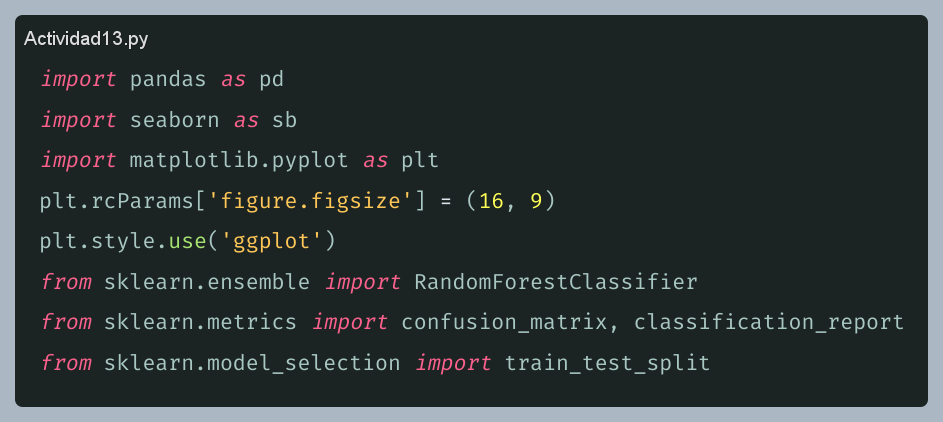
\includegraphics[width=90mm]{2025-03-31-10-32-53.png}
    \caption{Essential imports.}
\end{figure}

\newpage
\subsection{Before creating the model}
Now, we parse the .csv file as a Pandas dataframe and perform a holdout cross-validation where we will assign 70\% of our dataset to the training set.
\begin{figure}[h]
    \centering
    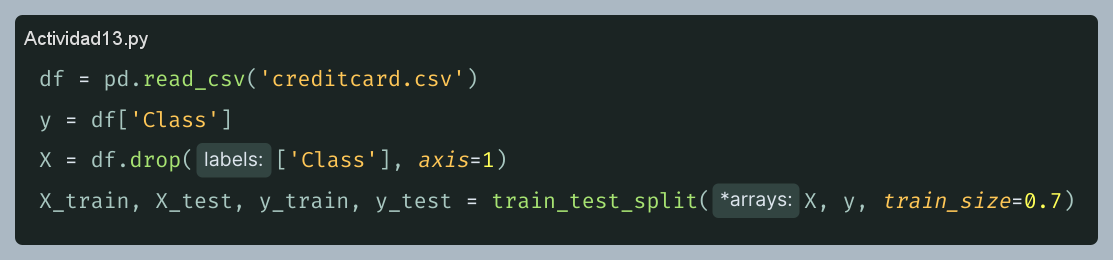
\includegraphics[width=90mm]{2025-03-31-10-36-08.png}
    \caption{Splitting the dataset into training examples and testing examples.}
\end{figure}
\begin{figure}[h]
    \centering
    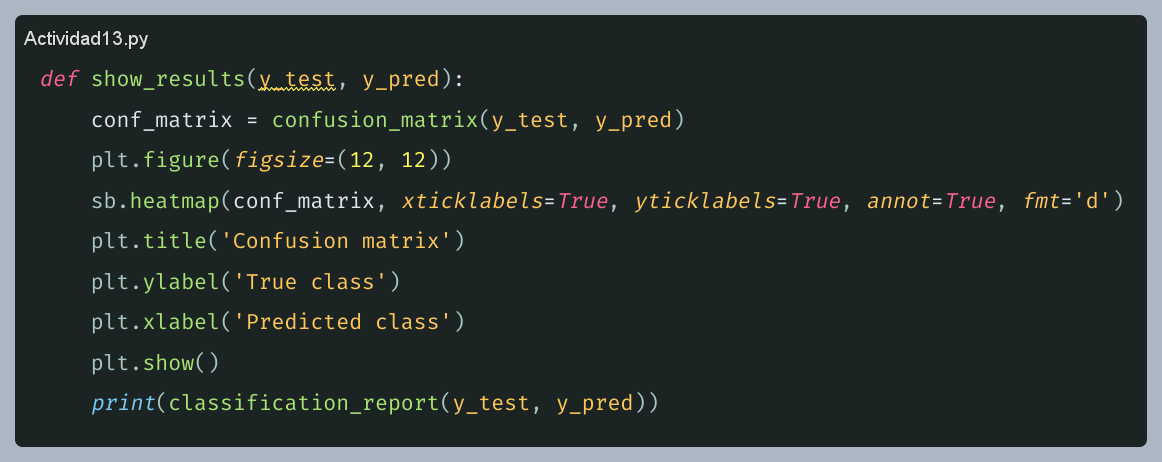
\includegraphics[width=90mm]{2025-03-31-10-39-22.png}
    \caption{Function to show the model results.}
    \label{fig:function}
\end{figure} \par
Then, we define a function that we will use to print out the model results as shown in Figure \ref{fig:function}.

\subsection{Creating the model}
Finally, we create the model using the following hyperparameters:
\begin{itemize}
    \item Generate 100 trees.
    \item Use different training sample sizes.
    \item The maximum quantity of features for each tree will be determined by the square root of the total features.
    \item Will use 8 cores of our CPU to make training faster.
    \item Emulate cross-validation in trees to avoid overfitting.
\end{itemize}
\begin{figure}[h]
    \centering
    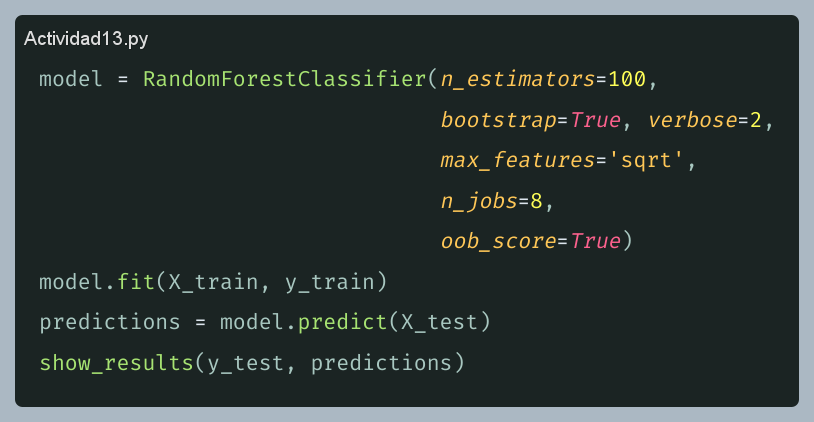
\includegraphics[width=90mm]{2025-03-31-10-58-02.png}
    \caption{Creation of the random forest classifier model.}
\end{figure}

\newpage
\section{Results}
After training the model for almost a minute, we get the following heatmap for the model
\begin{figure}[h]
    \centering
    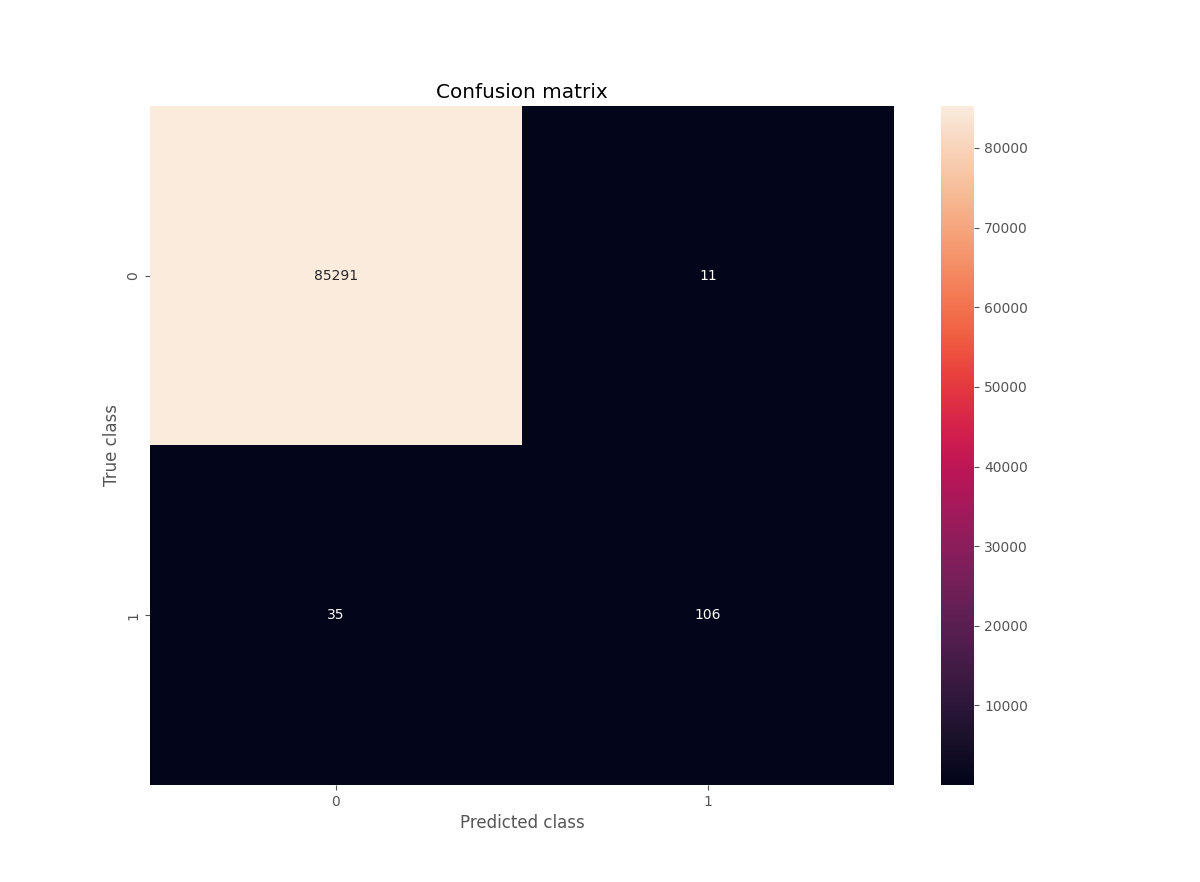
\includegraphics[width=110mm]{heatmap.png}
    \caption{Heatmap for predictions vs real examples.}
\end{figure}
We can see very good results for this model with only 46 mistakes in all predictions made. Also, the f1-score macro average is 0.91, which is an excellent result. This means that we built a good model even if the dataset was very unbalanced.

\section{Conclusions}
The Random Forest classifier implemented in this study has demonstrated outstanding performance in detecting credit card fraud, achieving an f1-score macro average of 0.91 and making only 46 misclassifications across the entire test set. These results are particularly impressive considering the highly unbalanced nature of the dataset, which typically poses significant challenges for classification algorithms. \par
The success of our model can be attributed to several key factors. First, the inherent ensemble approach of Random Forest effectively mitigated the risk of overfitting that would likely have occurred with a single decision tree model. Second, the hyperparameter configuration—including 100 trees, bootstrap sampling, and limiting features to the square root of the total feature count—provided an optimal balance between model complexity and generalization capability. Finally, the parallel processing across 8 CPU cores significantly reduced the computational time required for training this complex model. \par
Our findings confirm the advantages of Random Forest highlighted in the introduction, particularly its strong performance without extensive hyperparameter tuning and its resistance to overfitting. Despite the computational cost being higher than a single decision tree, the substantial improvement in classification accuracy justifies this trade-off for critical applications like fraud detection. \par
Future work could explore additional techniques to further enhance model performance, such as addressing class imbalance through resampling methods, feature engineering beyond PCA-transformed variables, or comparing Random Forest performance against other ensemble approaches like gradient boosting. Nevertheless, this implementation demonstrates that Random Forest is a powerful and effective tool for credit card fraud detection, capable of delivering high-quality predictions even with challenging, real-world financial datasets.

\bibliographystyle{../common_styles/cs-agh}
\bibliography{act13_bibliography}

\end{document}